\section{The AMIDST modelling framework}\label{section:AMIDSTmodelClass}

One of the main goals of the AMIDST project is the definition of a general modelling framework with the following characteristics: 

\begin{itemize}
\item \textbf{Feature 1:} it should be applicable to the three considered use cases, i.e., Daimler, Cajamar and Verdande;

\item \textbf{Feature 2:}  it should be general enough to be applicable to any future, potentially similar, use cases;

\item \textbf{Feature 3:} it should allow the integration of domain/expert knowledge about the structure of the process being modelled, and

\item \textbf{Feature 4:} it should be scalable, supporting both inference and learning from massive data streams.

\end{itemize}


%When designing this model class, we also tried to define a model family that eases as much as possible the integration of domain/expert knowledge, which is a common place in the different application scenarios discussed in Section \ref{Section:PreliminaryModels}.

The AMIDST modelling framework has been designed with the goal of meeting these four requirements. It is introduced in
the following two sections. In Section \ref{StaticFramework}, we firstly discuss the static modelling framework that
covers the static models presented in the related application scenarios. In Section \ref{GeneralModelClass}, we
introduce the general AMIDST modelling framework as a dynamic extension of the previous static modelling framework. As
proof of concept of the generality of this modelling framework, we show how the framework can be instantiated to solve each of the application scenarios of the different use cases. The graphical notation introduced in Section \ref{SubSection:GraphicalNotation} will be employed when describing these probabilistic graphical models. Finally, a summary with a higher level view of the AMIDST modelling framework is included in Section \ref{summaryAMIDSTModels}.

%Taking these different characteristics into account and using the graphical notation introduced in Section \ref{SubSection:GraphicalNotation}, the general AMIDST model class, as well as its specific instantiations to each use case, are introduced and discussed in Section \ref{GeneralModelClass}. A summary with a higher level view of the AMIDST model class is finally included in Section \ref{summaryAMIDSTModels}.

%-----------------------------------------------------------------------------------------------------------------------------------------
\subsection{The static modelling framework}\label{StaticFramework}
%-----------------------------------------------------------------------------------------------------------------------------------------

Figure \ref{Figure:StaticModellingFramework} visually shows the proposed static modelling framework. This general model
is the result of combining the high-level structure of the static models described for two of the application scenarios discussed in Section \ref{Section:PreliminaryModels}. This static modelling framework has been designed having in mind that it should be easily extendable to a dynamic context. As it can be seen, subnetworks have been used to group variables with similar properties, so that the commonalities between all models are taken into account. 

\begin{figure}[ht!]
\begin{center}
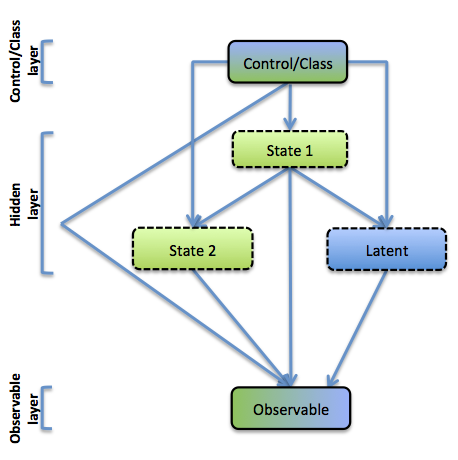
\includegraphics[scale=0.4]{./figures/StaticModellingFramework}
\caption{\label{Figure:StaticModellingFramework} The static modelling framework.}
\end{center}
\end{figure}

The first main characteristic of this static model is that all the modelling variables are structured in three different
layers, each one with distinct semantics. We believe that this layered division of the modelling variables can
help facilitate the integration of domain/expert knowledge. These three layers can be described as follows:


\begin{itemize}

\item \textbf{Control/class layer:}  This upper layer can be instantiated as a target variable for classification
  models. Alternatively, it can  act as a ``control'' layer, by containing specific variables in the systems that
  directly or causally influence the rest of the variables in the model. This ``control'' interpretation will gain significance in the dynamic context.

The layer is represented by a subnetwork including either continuous or discrete observed variables. The links from the
continuous observed variables to the state subnetworks in the \textit{Hidden layer} (i.e., the set of ``State 1'' and
``State 2'' variables) will possibly be handled with logit and probit functions.

\item \textbf{Hidden layer:}  This layer attempts to capture those parts of the system/process that can not be directly
  observed or measured, but which is believed (e.g.\ based on domain/expert knowledge) to be part of the system/process. Moreover, we can also use this layer as a way to capture complex conditional dependencies and distributions (e.g. mixture of Gaussians) that might be present between variables in the observable layer. 

This layer is structured as a set of interconnected discrete and continuous hidden subnetworks, for which only links from discrete to continuous subnetworks are allowed. We will use the term \textit{state} variables to refer to the set of discrete hidden variables in both ``State 1'' and ``State 2'' subnetworks, and the term \textit{latent}\footnote{The term \textit{latent} for variables is generally used in statistics to refer to hidden variables as opposed to observed ones. However, we will use it here to exclusively refer to continuous hidden variables.} variables to refer to the set of continuous hidden variables in the ``Latent'' subnetwork. The distinction between the subnetworks ``State 1'' and ``State 2'' will be better understood in the dynamic context. 

\item \textbf{Observable layer:} This layer accounts for those variables modelling the part of the system/process that can be observed/measured. These observations are conditioned on the variables in the above two layers. 

This layer is represented by a subnetwork including both discrete and continuous observed variables. These variables can in principle be interconnected but, in our different use cases, only links from discrete to continuous nodes are required. However, in general, we would not need to restrict the direction of the links between the variables in this layer.

\end{itemize} 


According to the discussions in Section \ref{Section:PreliminaryModels} on the distribution families governing the use
cases, we have designed a modelling framework that can be parametrized in alternative ways to improve the expressibility
and applicability to different problem domains. This parametrization is also influenced by the possible impact it can
have in the inference and learning algorithms. In general, this modelling framework falls inside the conditional linear
Gaussian framework, and so the conditional probability distributions are parameterized as detailed in Section
\ref{SubSection:HybridBNs}. On the other hand, the modelling framework might also contain instantiations which are not
covered by this general CLG framework. More precisely, when the top layer class is instantiated to  a continuous
subnetwork, then the conditional probabilities of ``State 1'' and ``State 2'' may be instantiated with logistic or
probit distributions, because we encounter continuous parents with discrete children. Additionally, we also envision the
possibility of introducing in the observable layer, the use of probability distributions belonging to the MOTBF family
\cite{Langseth12}, in order to extend the expressive power of the modelling framework (see Section \ref{SubSection:EmpiricalDistributions}).

Full details about how this framework can be instantiated to solve the different application scenarios will be given in the next section. But, as an illustrative example, we show in Figure \ref{Figure:StaticModellingInstantiations} how this static modelling framework can be instantiated to the static models presented for Daimler (see Section \ref{Section:Daimler:EarlyRecognition}) and Cajamar (see Section \ref{SubSection:Predicting}). In the case of Verdande, no static models has been considered. 


\begin{figure}[ht!]
\begin{center}
\begin{tabular}{cc}
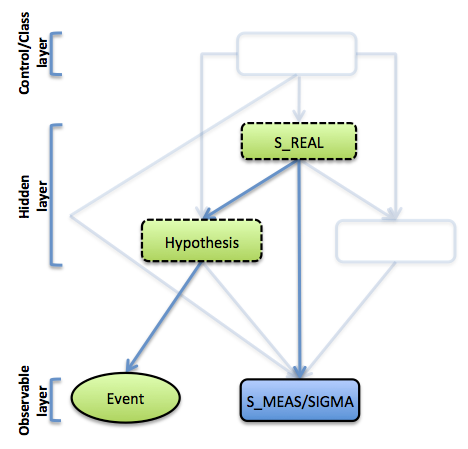
\includegraphics[scale=0.4]{./figures/DaimlerStaticModelling}
&
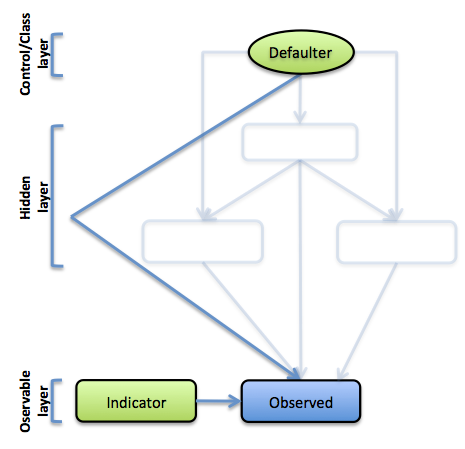
\includegraphics[scale=0.4]{./figures/CajaMarStaticModelling}
\\Daimler static model & Cajamar static model \\
\end{tabular}
\caption{\label{Figure:StaticModellingInstantiations} An illustrative example with instantiations of the static modelling framework for the Daimler and Cajamar static models, respectively.}
\end{center}
\end{figure}
%-----------------------------------------------------------------------------------------------------------------------------------------
\subsection{The general AMIDST modelling framework}\label{GeneralModelClass}
%-----------------------------------------------------------------------------------------------------------------------------------------

Figure \ref{Figure:AMIDSTModelClass} shows the proposed general AMIDST modelling framework. This general framework is the result of the temporal extension of the static modelling framework presented in the above section. It is also the result of combining all the dynamic models that have been previously defined for the different use cases. 

\begin{figure}[ht!]
\begin{center}
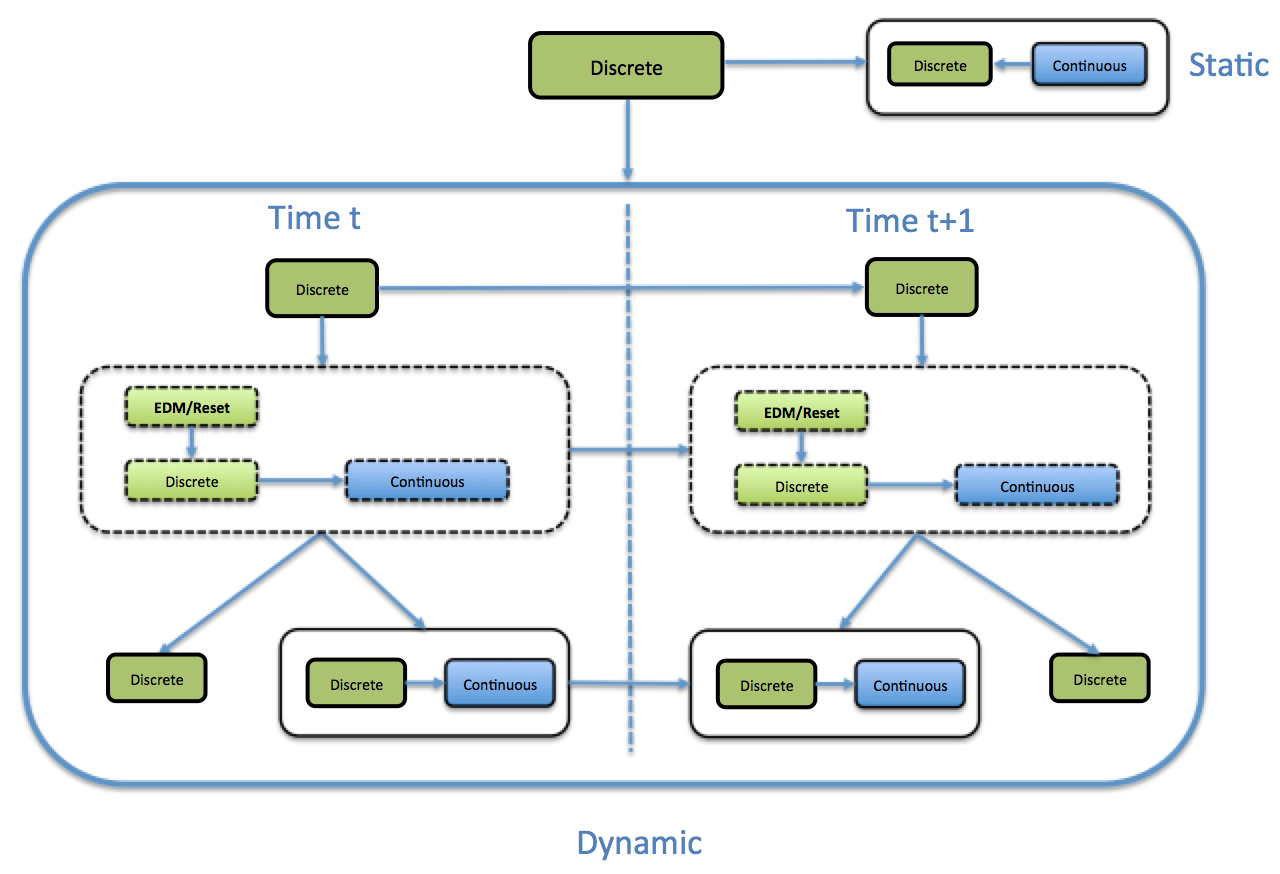
\includegraphics[scale=0.465]{./figures/AMIDSTModelClass}
\caption{\label{Figure:AMIDSTModelClass} The AMIDST modelling framework.}
\end{center}
\end{figure}

The general AMIDST modelling framework can be seen as a 2T-DBN (see Section \ref{SubSubSection:2DBNs}), i.e., it
satisfies the first order Markov property and the stationarity assumption. However, this model is not as general as a
2T-DBN as it has a more restricted internal structure that seeks to offer a  trade-off between expressiveness and efficiency. 

We should point out that the static modelling framework described in Section \ref{StaticFramework} can be seen as a
simple instantiation of this general model when the temporal dependencies are obviated. That is, when only one time slice of the 2T-DBN is considered. 

One of the main characteristics of this temporal extension is that the inter-time slice dependencies are only allowed
between variables in the same layer. At this stage, we have not found any strong argument to allow for more complex
instantiations. The three different layers maintain the same semantics as in the static case, although  they now can
also be interpreted from a dynamic point of view. We briefly comment on the main consequences: 

\begin{itemize}

\item \textbf{Control/class layer:} This layer can now be instantiated to support dynamic classification, i.e., we aim to predict a temporal sequence of labels rather than a single label. If it is instantiated as a control layer, it can be used to model the transition probabilities between the variables of the hidden layer. This can be seen as a modelling trick to relax the stationarity assumption and, hence, widen the applicability of the framework.

\item \textbf{Hidden layer:}  In the dynamic case, the hidden variables in this layer can be temporally connected. In
  this way, it is easy to see that our modelling framework subsumes the basic dynamic models commented in Section
  \ref{SubSection:DBNs}. As in the static case, these variables aim to capture the dynamic parts of the system that can
  not be observed but are nonetheless relevant for modelling the dynamic system/process. State and latent variables connected over time can be used to model a process that is evolving and changing over time.

As can be seen in Figure \ref{Figure:AMIDSTModelClass}, this layer can contain state variables that are not connected
over time (i.e., variables in ``State 2'' subnetwork), and which can be used, for instance, to model mixture of Gaussian distributions over the observed continuous variables in the \textit{Observable layer}. 

Recall that links from latent variables to state variables are not allowed, neither in the same time step nor between consecutive ones.

\item \textbf{Observable layer:}  Observed variables in this layer now have the possibility of being connected over time. Again, there is no restriction on the temporal links between continuous and discrete variables. 

\end{itemize} 



In the following sections, we will show how this modelling framework satisfies the aforementioned \textbf{Feature 1}, by
describing how each particular use case fits in this restricted 2T-DBN AMIDST model. This instantiation process of the
general AMIDST model to the three use cases (all of them with different application scenarios) can also be seen as a
practical example demonstrating the general applicability of the resulting AMIDST modelling framework. This provides
arguments in favour of \textbf{Feature 2} and shows how the AMIDST modelling framework can be potentially instantiated
to other future use cases. In our opinion, these different instantiations also show how the layer and component based
structure of this modelling framework might help ease the process of building other future models using domain/expert
knowledge, thereby giving support to \textbf{Feature 3}. Finally, the remaining task is related to
\textbf{Feature 4} and consists of designing inference and learning algorithms that enable the AMIDST
modelling framework to handle massive data streams. We can envision that this latter process might result in
modifications of some of the elements and assumptions of the proposed modelling framework, if this is needed to better balance the accuracy and
computational performance as required by the use-case providers.  



%-----------------------------------------------------------------------------------------------------------------------------------------
\subsubsection{Daimler model class}\label{daimlerAMIDSTModels}
%-----------------------------------------------------------------------------------------------------------------------------------------

Daimler's model class has been previously displayed in Figure \ref{Figure:daimlerLEdynGeneric}. Taking the general AMIDST modelling framework into account, Daimler's model class can be reinterpreted, according to Figure \ref{Figure:AMIDSTModelClassDaimler}, as follows:

\begin{figure}[ht!]
\begin{center}
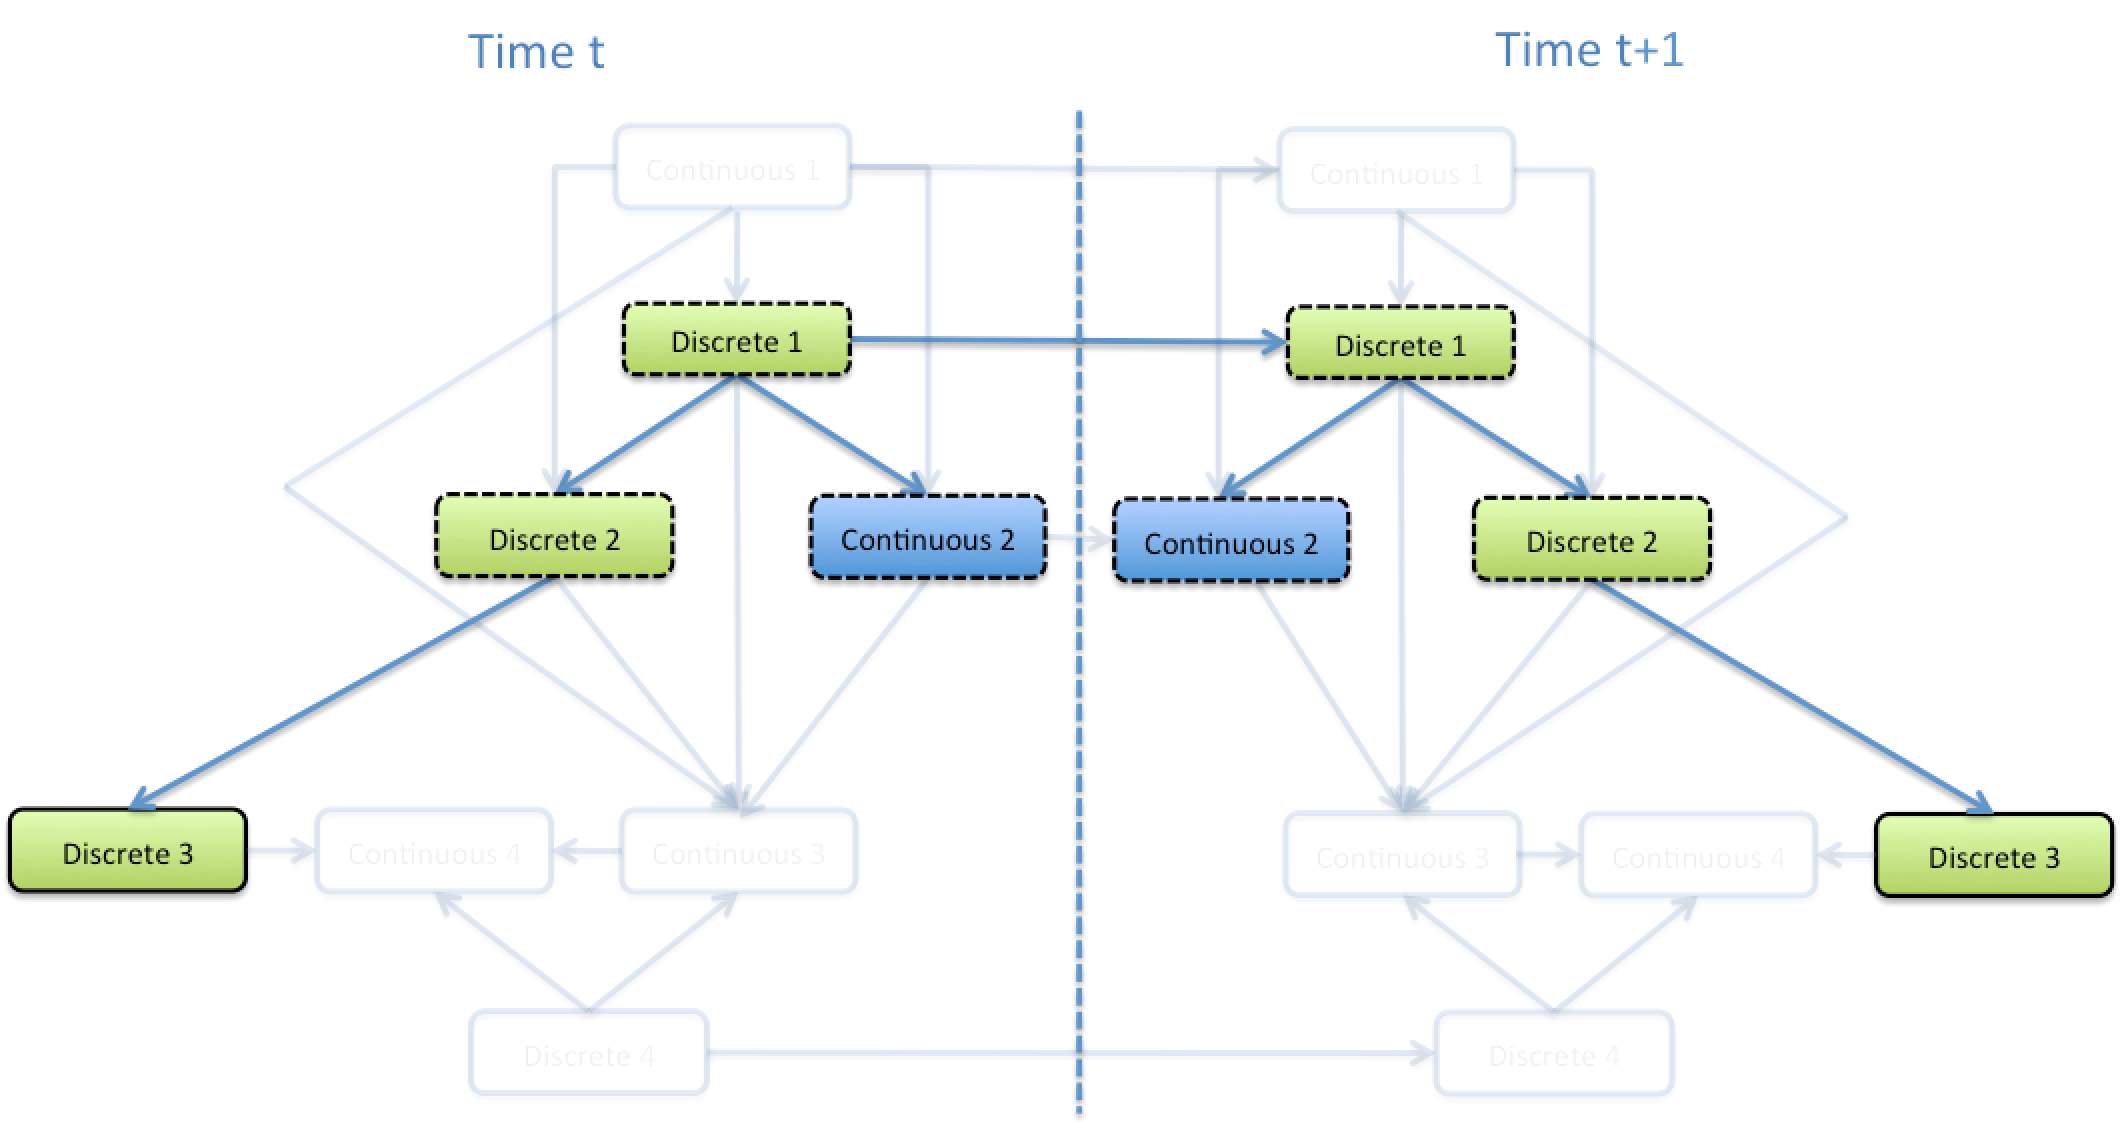
\includegraphics[scale=0.39]{./figures/AMIDSTModelClassDaimler}
\caption{\label{Figure:AMIDSTModelClassDaimler} AMIDST modelling framework - Daimler}
\end{center}
\end{figure}

\begin{itemize}

\item \textbf{Control/class layer}: It is not used in this domain.

\item \textbf{Hidden layer}: The two sets of state variables are required in this layer. 

The lower set of state variables (i.e., ``State 2'' subnetwork in Figure \ref{Figure:AMIDSTModelClass}) encodes a polytree \cite{JensenNielsen2007} for the hierarchy of the Hypothesis. This polytree structure, not explicitly encoded in the model, can indeed be exploited during inference.

Connections through time slices are only made at the top level state variables (i.e., ``State 1'' subnetwork in Figure
\ref{Figure:AMIDSTModelClass}), which corresponds to the signal real values (S\_REAL\footnote{Although these variables
  are inherently continuous, we notice that they are discretized to avoid the inference problems derived of having
  continuous parents with discrete children (see Section \ref{Section:DaimlerDynamic}).}). Consequently, the future and
past time slices of our 2T-DBN are conditionally independent given the S\_REAL variables corresponding to the present time. 

In addition, inside a time slice, the observed continuous and hidden discrete subnetworks are also conditionally
independent given the S\_REAL variables. In the case that we want to contemplate a possible extension in which lower
level Hypotheses are connected over time, then the ``State 1'' subnetwork would contain both the S\_REAL variables and the temporally linked Hypothesis. However, as commented before, this could greatly complicate the inference process. 

\item \textbf{Observable layer:} There are two sets of observed variables in this case. On the one hand, we encounter a group of variables representing the measured data (S\_MEAS), along with the variables encoding the sensor noise (S\_SIGMA). The resulting structure is again a polytree, which presents some advantages for the inference process. On the other hand, we have a single discrete node for the manoeuvre Event, which will be the target variable during inference. 

\end{itemize}

%-----------------------------------------------------------------------------------------------------------------------------------------
\subsubsection{Cajamar model class}\label{cajamarAMIDSTModels}
%-----------------------------------------------------------------------------------------------------------------------------------------

Concerning the Cajamar use case, both application scenarios share the same modelling structures (see Section \ref{Section:CajaMarModels}). The static approach, as discussed above, can be trivially seen as a particular case of the dynamic one. At this point, we focus on the dynamic model, since the general AMIDST modelling framework is primarily a dynamic model class. Thus, the high-level description of Cajamar's dynamic model (previously displayed in Figure \ref{fig:component}) can be reinterpreted according  to Figure \ref{Figure:AMIDSTModelClassCajamar}. 

\begin{figure}[ht!]
\begin{center}
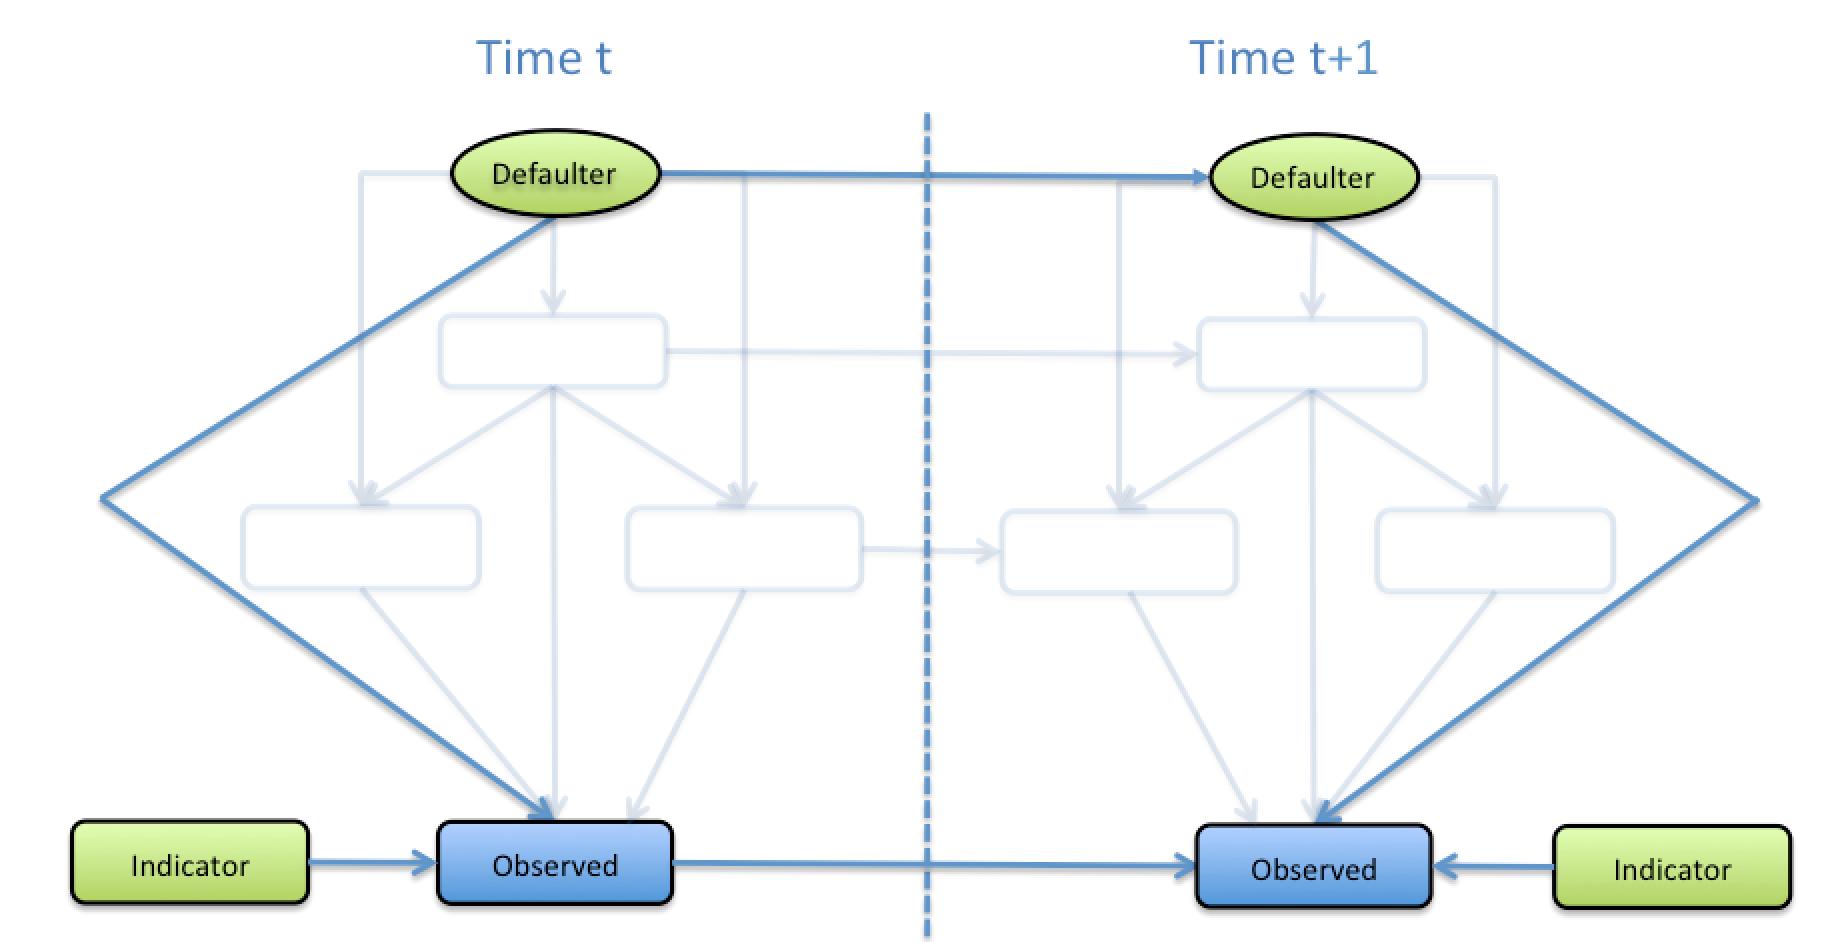
\includegraphics[scale=0.39]{./figures/AMIDSTModelClassCajamar.png}
\caption{\label{Figure:AMIDSTModelClassCajamar} AMIDST modelling framework - Cajamar.}
\end{center}
\end{figure}


Following the layer-wise analysis used above, Cajamar's model is described as follows:
\begin{itemize}

\item \textbf{Control/class layer}: The top node ``Defaulter" in this layer, represents the class variable to categorize a client as defaulter or non-defaulter. There exist temporal links between consecutive time steps to model the dynamic nature of being a defaulter or non-defaulter. Note that this is indeed the target variable in the inference process.

\item \textbf{Hidden layer}: It is not used in this domain.

\item \textbf{Observable layer:} The ``Observed" continuous subnetwork represents information corresponding to the socio-demographic variables, memory variables, financial activity, and past payment behaviour of a client, which, in principle, may or may not be connected over time. Moreover, the ``Indicator" discrete subnetwork includes the set of indicator discrete variables denoted as $\delta_{X_t}$. These indicator variables are used for modelling situations in which some variables in the ``Observed" continuous subnetwork have a large number of zeros.

\end{itemize}


%-----------------------------------------------------------------------------------------------------------------------------------------
\subsubsection{Verdande model class}\label{verdandeAMIDSTModels}
%-----------------------------------------------------------------------------------------------------------------------------------------

Figure \ref{Figure:AMIDSTModelClassVerdande} shows how the general AMIDST modelling framework is instantiated in the case of Verdande. This instantiated model encompasses the models of the three application scenarios previously discussed in Section \ref{Section:VerdandeModels} and depicted in Figures \ref{Figure:VTScenario1}, \ref{Figure:VTScenario2} and \ref{Figure:VTScenario3}.

\begin{figure}[ht!]
\begin{center}
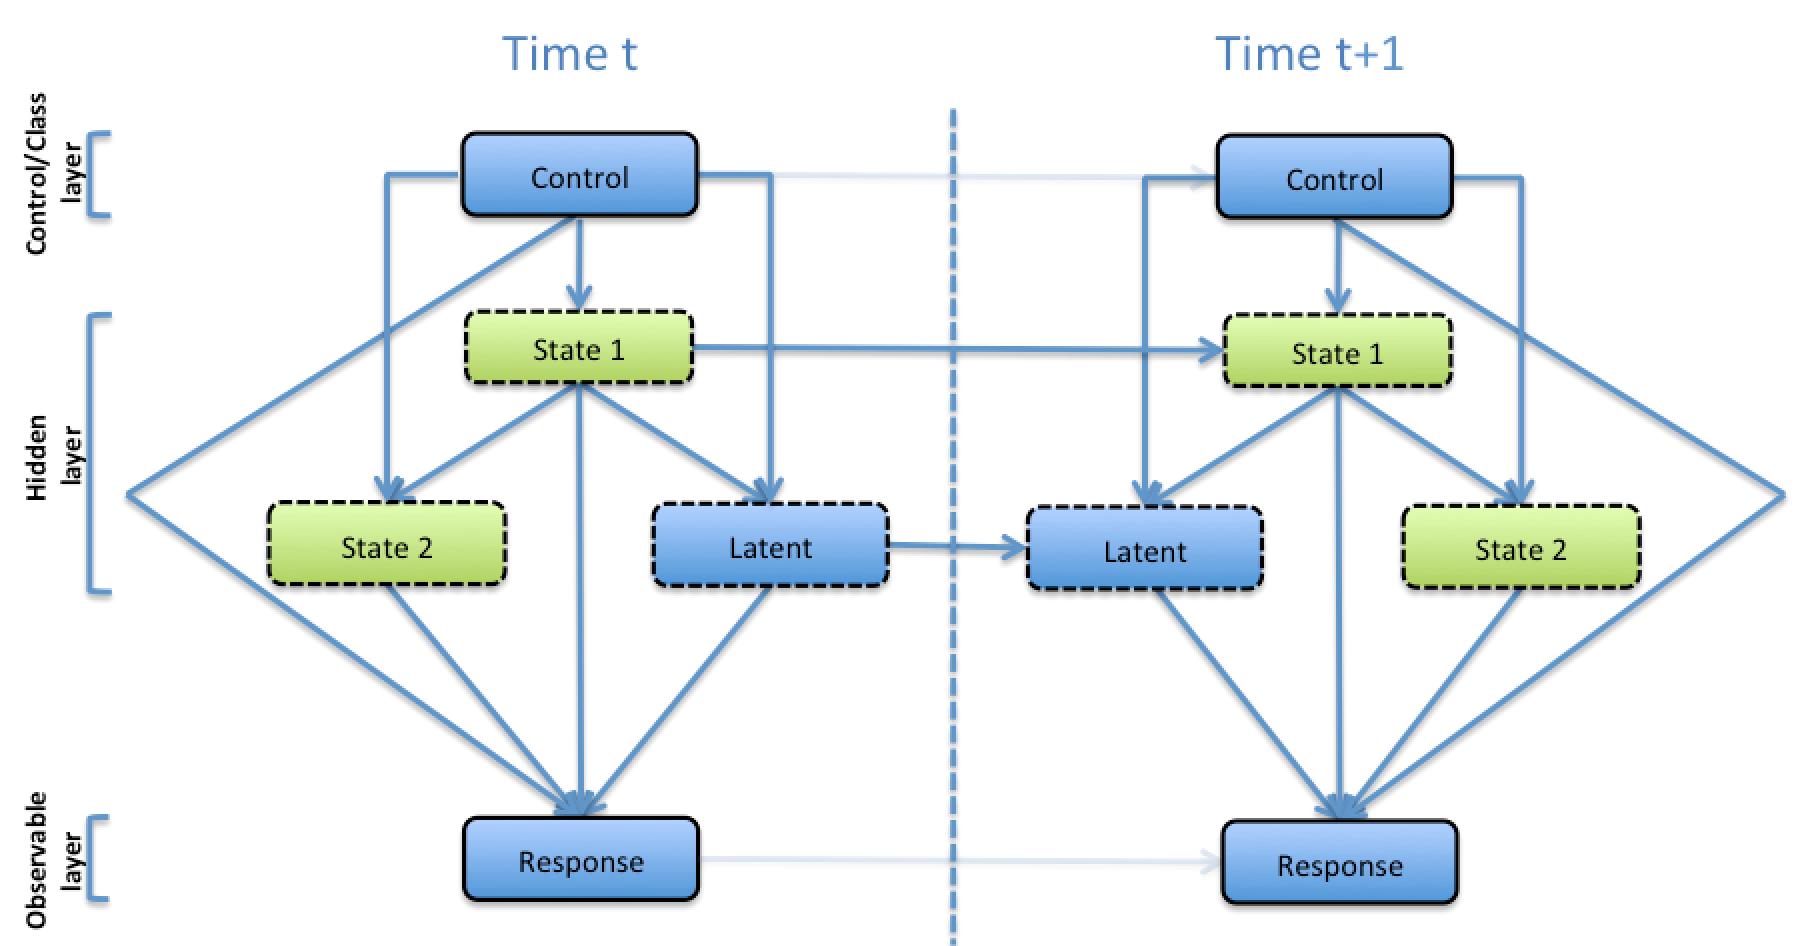
\includegraphics[scale=0.39]{./figures/AMIDSTModelClassVerdande}
\caption{\label{Figure:AMIDSTModelClassVerdande} AMIDST modelling framework - Verdande.}
\end{center}
\end{figure}

Verdande's model class can then be described as follows:

\begin{itemize}
\item \textbf{Control/class layer}:  This layer includes a subnetwork modelling the set of observed Control variables. In the three application scenarios, the role of these Control variables is to condition the transition probability of the state variables and also, to ensure the modelling of non-stationary transition probabilities.  

\item \textbf{Hidden layer}: This layer is directly instantiated from the general AMIDST modelling framework. However, there are some differences when applied to each particular application scenario:

\begin{itemize}
\item For the first application scenario (see Figure \ref{Figure:VTScenario1}):  ``State 2'' is not needed and ``State 1'' is instantiated to the ``Normal/Abnormal'' state variable. 

\item For the second application scenario (see Figure \ref{Figure:VTScenario2}): ``State 1'' is not needed and ``State 2'' is instantiated to a single multinomial variable whose role is to model mixture of Gaussians at the leaves. 

\item For the third application scenario (see Figure \ref{Figure:VTScenario3}): ``State 2'' is not needed and ``State 1'' is instantiated to a subnetwork containing the ``FormationNo'' and ``Switch'' variables.
\end{itemize}

\item \textbf{Observable layer:} For both application scenarios 1 and 3, this layer is instantiated as a single response variable; while for the application scenario 2, it may be instantiated as a set of (possibly interconnected) response variables. 
\end{itemize}

%-----------------------------------------------------------------------------------------------------------------------------------------
\subsection{Summary}\label{summaryAMIDSTModels}
%-----------------------------------------------------------------------------------------------------------------------------------------

As it has been shown in the previous sections, the proposed general AMIDST modelling framework of Figure \ref{Figure:AMIDSTModelClass} encompasses the different application scenarios of the three use cases, both for static and dynamic contexts. These three use cases come from very different domains: automotive, finance and oil-drilling. In our opinion, these are strong arguments in favour of the generality and applicability of this modelling framework. 

A higher level view of our proposed AMIDST modelling framework is displayed in Figure
\ref{Figure:AMIDSTModelClassHighLevel}. As commented before, it shows how the AMIDST modelling framework could actually
be seen as a ``restricted" 2T-DBN. It is restricted in three different ways. Firstly, all the nodes are structured in
three layers, each one with clear semantics while modelling: Broadly speaking, the \textit{control/class layer} either
represents control variables that may affect the stationary assumption, or represents the class variable in
classification tasks; the \textit{hidden layer} includes a sufficiently rich set of hidden variables to capture the
process dynamics and enhance the modelling capabilities; and the \textit{observable layer} encompasses the observable
variables such as sensor measurements or predictive attributes. The second restriction states that, as opposed to
general 2T-DBNs, the variables in this model class can only be temporally linked to other variables in the same
layer. Finally, the third and last restriction  states that continuous hidden variables cannot point to discrete (hidden
or observed) nodes. This last constraint implies that our inference algorithms will not have to deal with the hard and
open problem of computing posterior distributions or marginalize over continuous variables which are parents of discrete
children nodes. So, in most of the cases, the network can be parameterized using the conditional linear Gaussian
framework. In the particular case where this is not possible, because the instantiated model contains continuous parents
with discrete children, we have that the continuous nodes are always observed. 

\begin{figure}[ht!]
\begin{center}
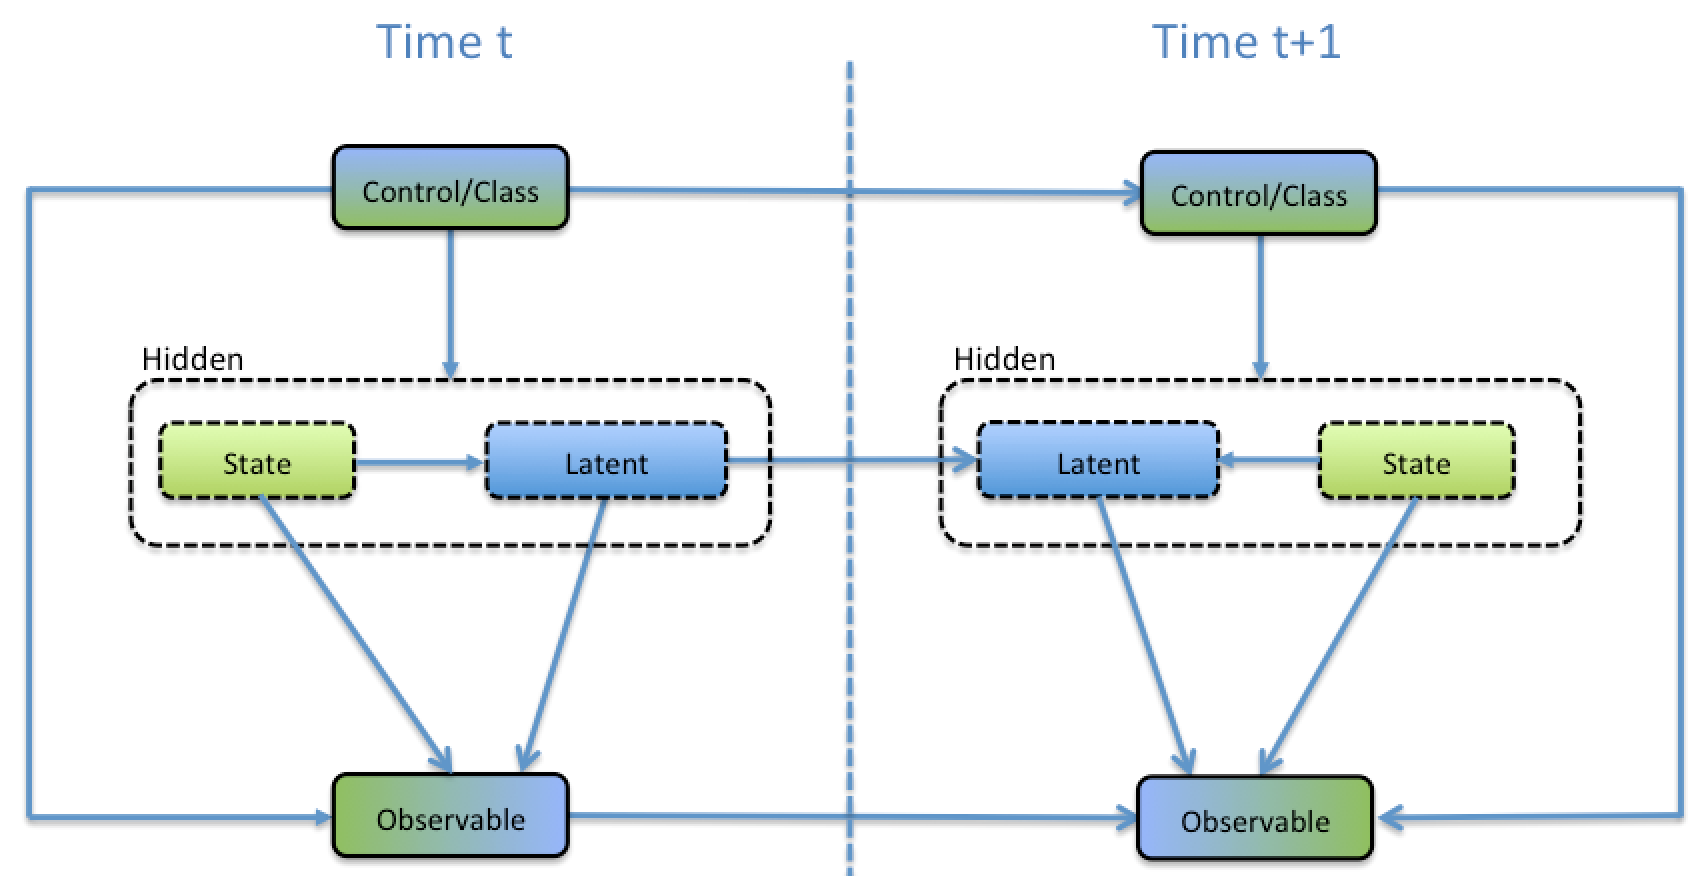
\includegraphics[scale=0.4]{./figures/AMIDSTModelClassGeneral}
\caption{\label{Figure:AMIDSTModelClassHighLevel} The high-level AMIDST modelling framework}
\end{center}
\end{figure}



